\documentclass{article}

\usepackage[utf8]{inputenc}
\usepackage[a4paper, total={6.3in, 8.8in}]{geometry}
\usepackage{amsmath}
\usepackage{bm}
\usepackage{amsfonts}
\usepackage{graphicx}
\usepackage{amssymb}  % assumes amsmath package installed
\usepackage{graphics} % for pdf, bitmapped graphics files
\usepackage{caption}
\usepackage{subcaption}
\usepackage{todonotes}
\usepackage{titling}
\newcommand{\subtitle}[1]{%
  \posttitle{%
    \par\end{center}
    \begin{center}\large#1\end{center}
    \vskip0.5em}%
}

\title{Exercise Session 2: Function Estimation and Time Series Prediction}
\subtitle{Support Vector Machines - Final Report}
\author{Victor van Wymeersch - R0690930}
\date{May 2022}

\begin{document}

\maketitle

    % \begin{figure}
    %     \centering
    %     \includegraphics[width=0.95\textwidth]{figures/}
    %     \caption{}
    %     \label{fig:}
    % \end{figure}
    
    % \begin{figure}[h]
    %      \centering
    %      \begin{subfigure}[b]{0.8\textwidth}
    %          \centering
    %          \includegraphics[width=\textwidth]{figures/}
    %          \caption{}
    %          \label{fig:}
    %      \end{subfigure}
    %      \hfill
    %      \begin{subfigure}[b]{0.8\textwidth}
    %          \centering
    %          \includegraphics[width=\textwidth]{figures/}
    %          \caption{}
    %          \label{fig:}
    %      \end{subfigure}
    %     \caption{}
    % \end{figure}
    
\section{Exercises} 
    \subsection{Support vector machine for function estimation} 
    
        % Effect of e 
        \begin{figure}[h]
             \centering
             \hspace{0.05\textwidth}
             % E = small 
             \begin{subfigure}[b]{0.4\textwidth}
                 \centering
                 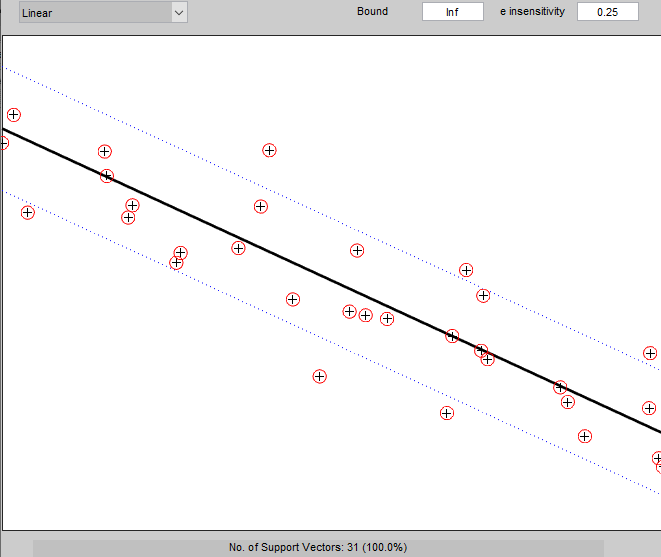
\includegraphics[width=\textwidth]{Assignment 2/figures/1_1/linear_b_inf_e_0_25.png}
                 \caption{e=0.25}
                 \label{fig:linear_small_e}
             \end{subfigure}
             \hfill
            % E = large
             \begin{subfigure}[b]{0.4\textwidth}
                 \centering
                 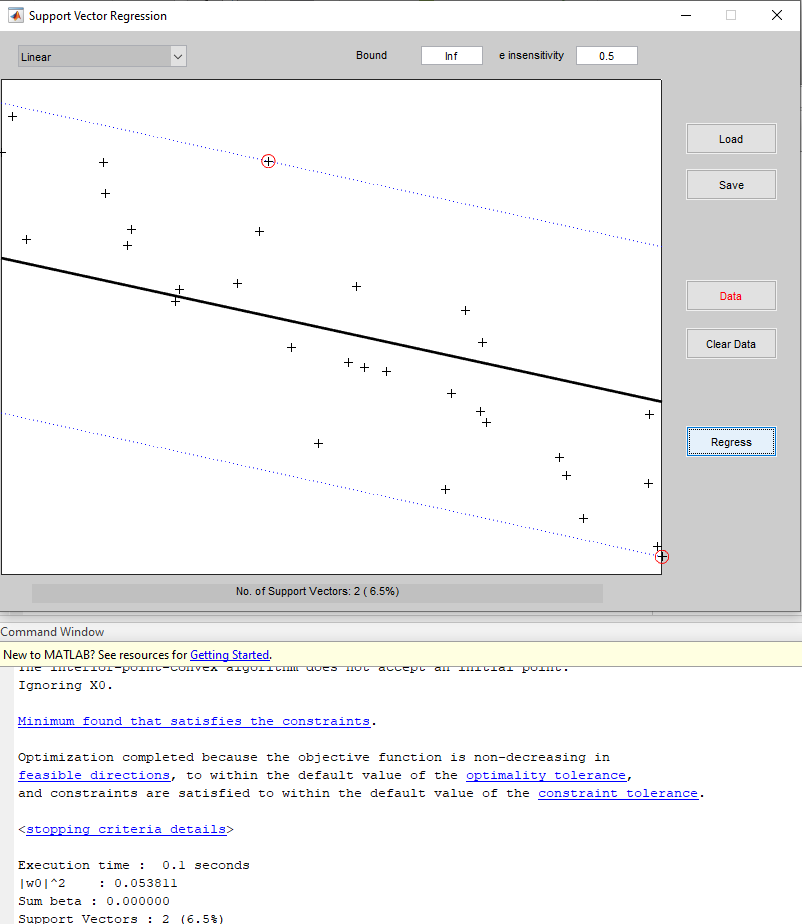
\includegraphics[width=\textwidth]{Assignment 2/figures/1_1/linear_b_inf_e_0_5.png}
                 \caption{e=0.5}
                 \label{fig:linear_large_e}
             \end{subfigure}
             \hspace{0.05\textwidth}
            \caption{Linear classification boundary in response to different values of e. }
        \end{figure}
        
        \begin{enumerate}
            \item e small: $|w0|^2$ =0.38, beta=0.01
            \item e large: $|w0|^2$ = 0.05, beta=0.00
        \end{enumerate}
    
    
        % Effect of bound on RBF classification linear 
        \begin{figure}[h]
             \centering
             % bound small - underfitting 
             \begin{subfigure}[b]{0.3\textwidth}
                 \centering
                 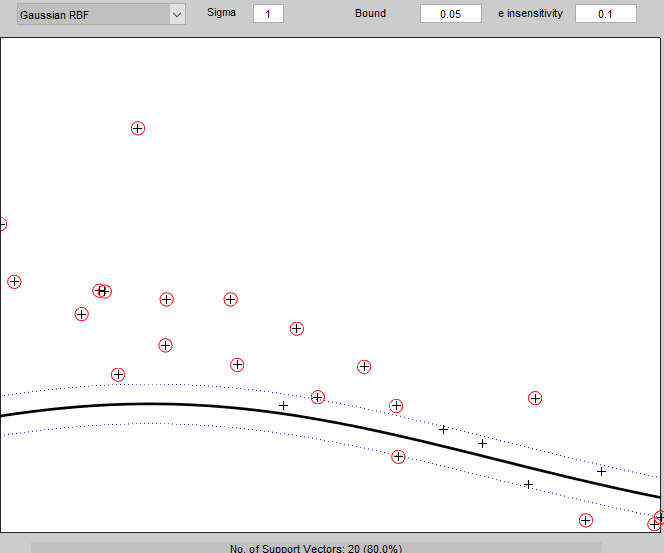
\includegraphics[width=\textwidth]{Assignment 2/figures/1_1/rbf_bound_small.png}
                 \caption{Under-fitting}
                 \label{fig:rbf_small_bound}
             \end{subfigure}
             \hfill
             % bound medium - fitted 
             \begin{subfigure}[b]{0.3\textwidth}
                 \centering
                 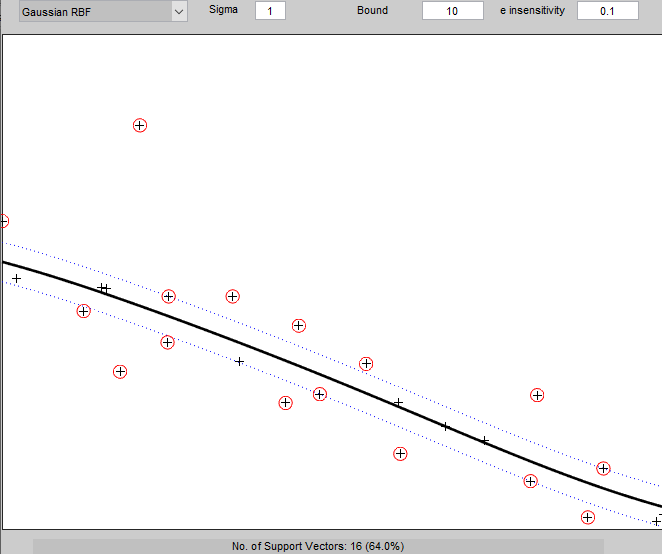
\includegraphics[width=\textwidth]{Assignment 2/figures/1_1/rbf_bound_medium.png}
                 \caption{Correctly fitted}
                 \label{fig:rbf_medium_bound}
             \end{subfigure}
             \hfill
             % bound large - over-fitted  
             \begin{subfigure}[b]{0.3\textwidth}
                 \centering
                 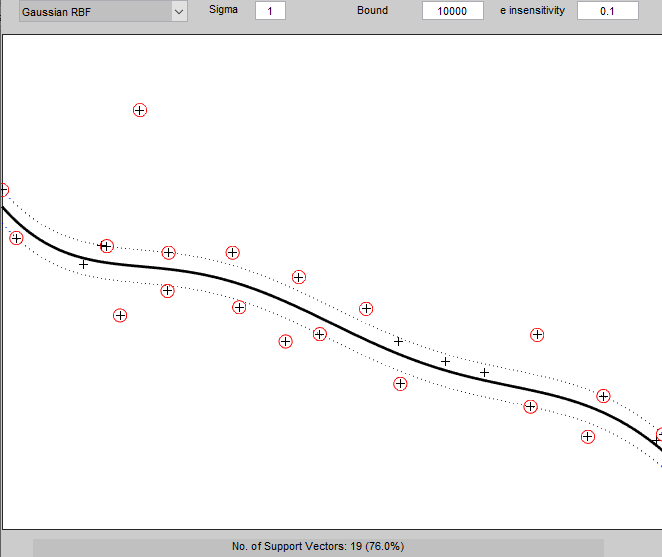
\includegraphics[width=\textwidth]{Assignment 2/figures/1_1/rbf_bound_large.png}
                 \caption{Over-fitting}
                 \label{fig:rbf_medium_bound}
             \end{subfigure}
            \caption{Effect of varying bound for regression on a linear dataset using a RBF kernel.}
        \end{figure}
        
        \begin{enumerate}
            \item Under: $|w0|^2$ = 0.42, beta=0.64
            \item proper: $|w0|^2$ = 2.34, beta=1.57
            \item over:$|w0|^2$ = 303.97, beta=6.79
        \end{enumerate}
        
        % Nonlinear dataset
        \begin{figure}[h]
             \centering
            % RBF kernel 
             \centering
             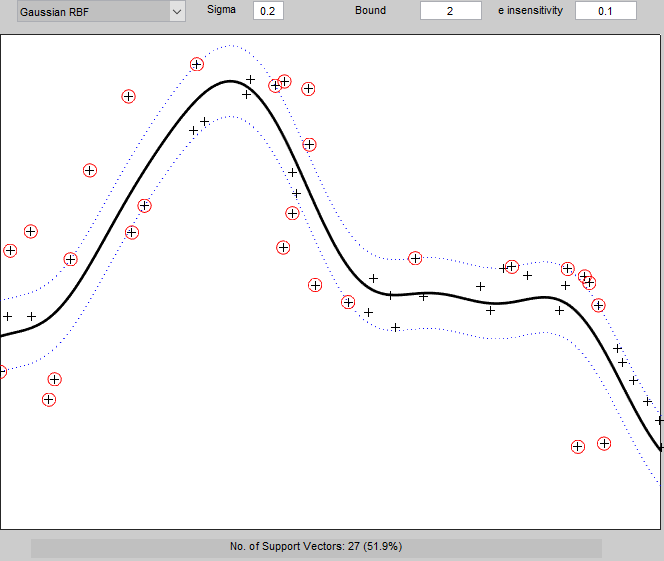
\includegraphics[width=0.5\textwidth]{Assignment 2/figures/1_1/gauss_rbf_sig_0_2_b_2_e_0_1.png}
             \label{fig:gauss_rbf}
            \caption{Regression results for Gaussian RBF kernels on a nonlinear dataset.}
        \end{figure}
        
        \begin{enumerate}
            \item guass rbf: $|w0|^2$ =1.89, beta=2.43
        \end{enumerate}
    
    \subsection{A simple example: the sinc function}
    
        \subsubsection{Regression of the sinc function}
            % Manual tuning of hyperparameters 
            \begin{figure}[h]
                 \centering
                 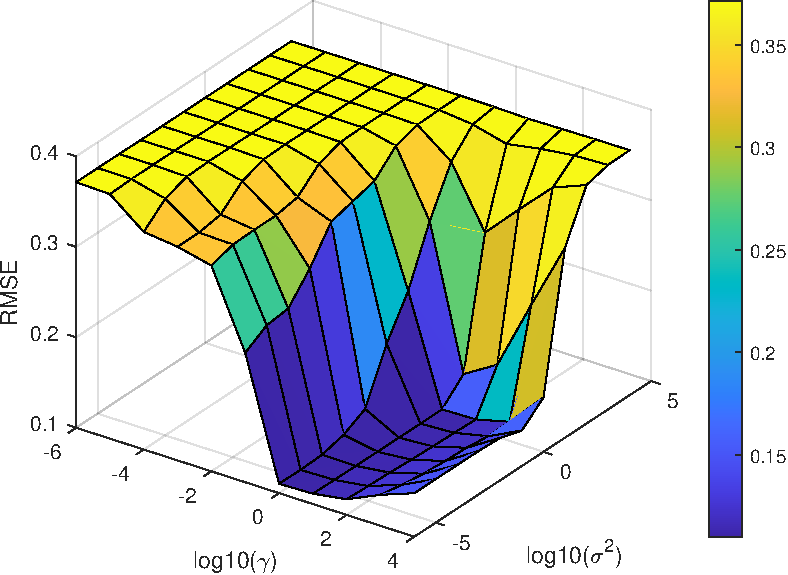
\includegraphics[width=0.5\textwidth]{Assignment 2/figures/1_2/hyper_tuning_results.pdf}
                 \label{fig:gauss_rbf}
                \caption{RMSE for varying $\sigma^2$ and $\gamma$ hyperparameters during regression of the Sinc function.}
            \end{figure}
            
            
             % Simplex and Gridsearch tuning results
            \begin{figure}[h]
                 \centering
                 \hspace{0.05\textwidth}
                 % simplex
                 \begin{subfigure}[b]{0.4\textwidth}
                     \centering
                     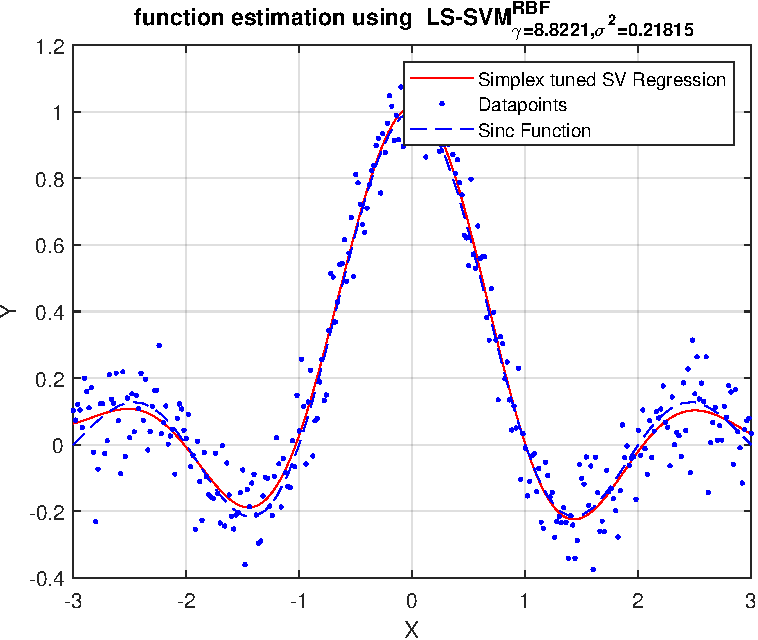
\includegraphics[width=\textwidth]{Assignment 2/figures/1_2/rbf_tuning_results_simp.pdf}
                     \caption{Simplex}
                     \label{fig:regression_simplex_tuned}
                 \end{subfigure}
                 \hfill
                % gridsearch
                 \begin{subfigure}[b]{0.4\textwidth}
                     \centering
                     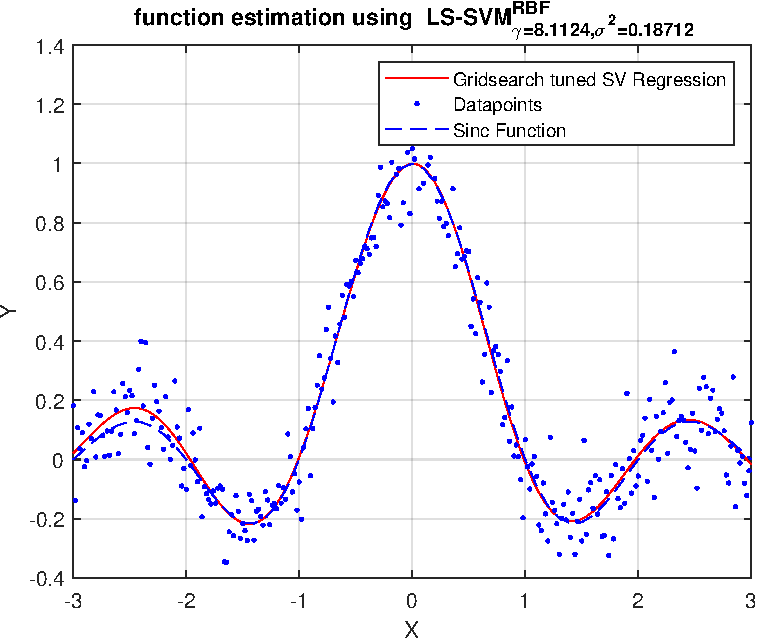
\includegraphics[width=\textwidth]{Assignment 2/figures/1_2/rbf_tuning_results_grid.pdf}
                     \caption{Gridsearch}
                     \label{fig:regression_grisearch_tuned}
                 \end{subfigure}
                 \hspace{0.05\textwidth}
                \caption{Regression on the Sinc function with RBF kernel tuned with hyperparameters tuned with different algorithms.}
            \end{figure}
            --
            Search method: SIMPLEX
              Gamma = 8.82, Sigma = 0.22 --, Error = 0.11
            --
            Search method: Gridsearch
              Gamma = 36422, Sigma = 0.91 --, Error = 0.11
        
        \subsubsection{Application of the Bayesian framework}
            % Bayesian framework for parameter tuning and regression 
            \begin{figure}[h]
                 \centering
                 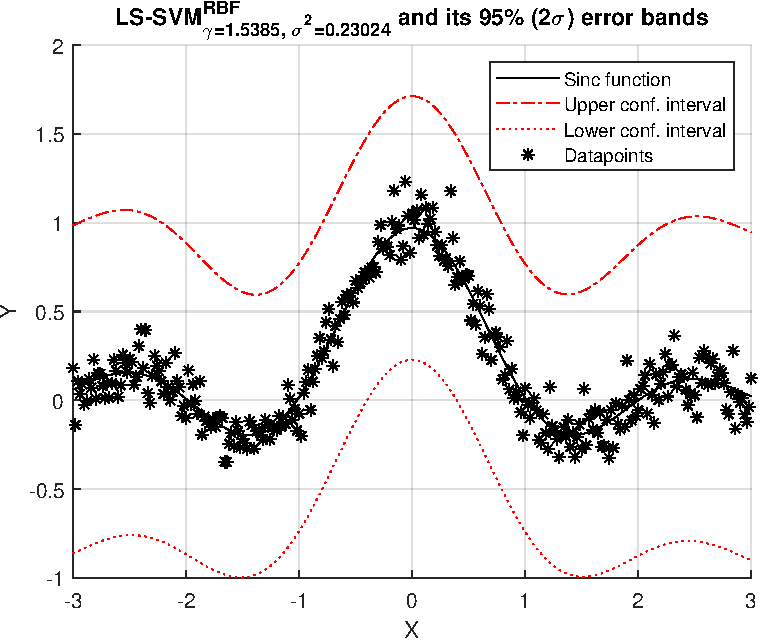
\includegraphics[width=0.5\textwidth]{Assignment 2/figures/1_2/bayesian_regression.pdf}
                 \label{fig:bayesianregression_sinc}
                \caption{Bayesian SVM regression of the Sinc function. }
            \end{figure}
        
    \subsection{Automatic Relevance Determination}
        % ARD
        \begin{figure}[h]
             \centering
             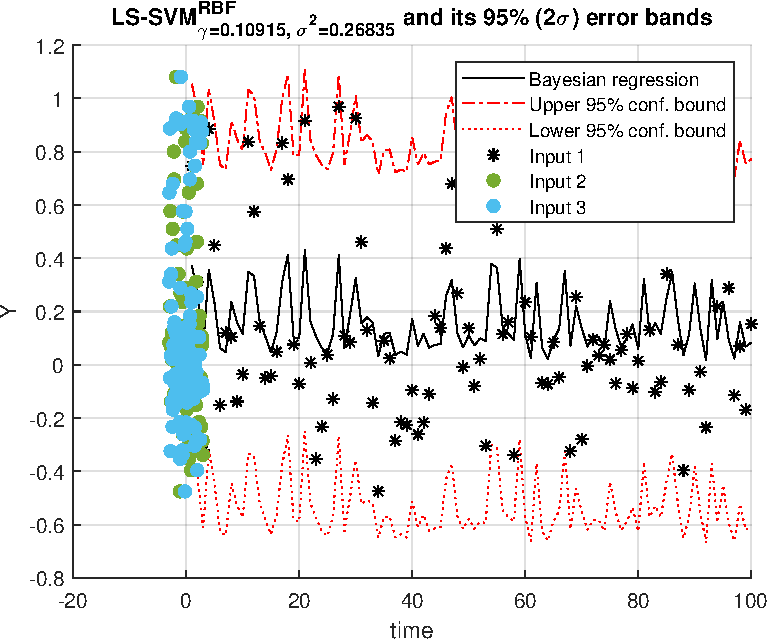
\includegraphics[width=0.5\textwidth]{Assignment 2/figures/1_3/bayesian_regression.pdf}
             \label{fig:bayesianregression_ard}
            \caption{Automatic relevance determination using the Bayesian framework. }
        \end{figure}
            
            
    \subsection{Robust regression}
        % Robust vs nonrobust regression 
        \begin{figure}[h]
             \centering
             \hspace{0.05\textwidth}
             % robust
             \begin{subfigure}[b]{0.4\textwidth}
                 \centering
                 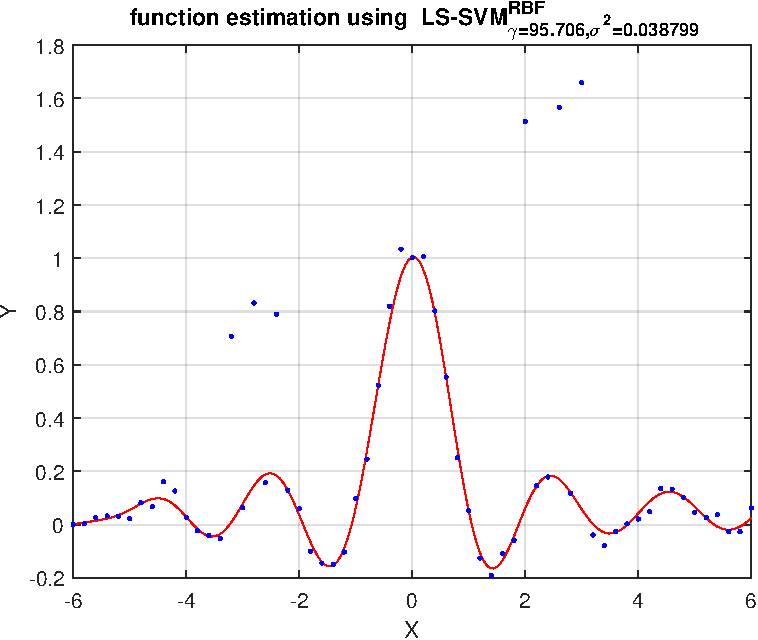
\includegraphics[width=\textwidth]{Assignment 2/figures/1_4/robust_mae_whuber.pdf}
                 \caption{Robust regression}
                 \label{fig:robust_regression}
             \end{subfigure}
             \hfill
            % Non robust
             \begin{subfigure}[b]{0.4\textwidth}
                 \centering
                 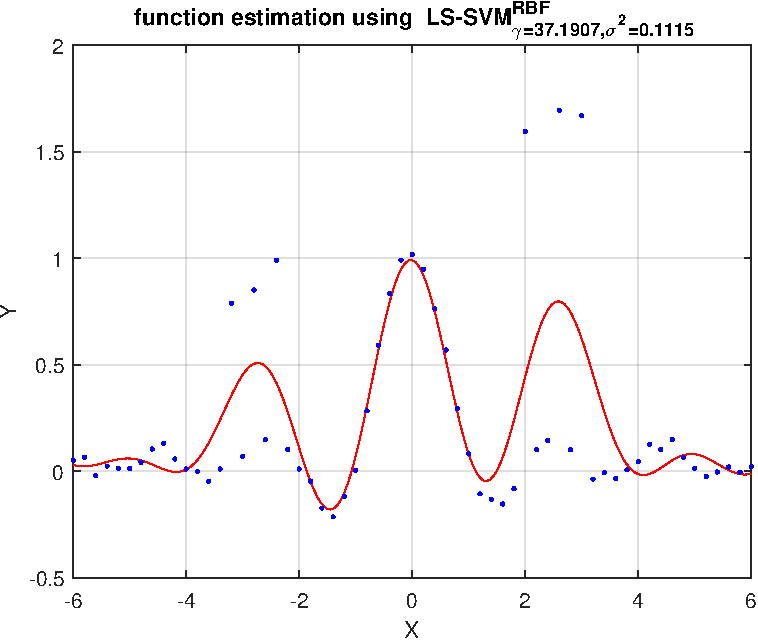
\includegraphics[width=\textwidth]{Assignment 2/figures/1_4/standard_mse.pdf}
                 \caption{Non-robust regression}
                 \label{fig:non_robust_regression}
             \end{subfigure}
             \hspace{0.05\textwidth}
            \caption{Robust vs non-robust regression in the presence of noise on the Sinc function. }
        \end{figure}
        
        
        % Robust regression function comparison
        \begin{figure}[h]
             \centering
             % huber
             \begin{subfigure}[b]{0.22\textwidth}
                 \centering
                 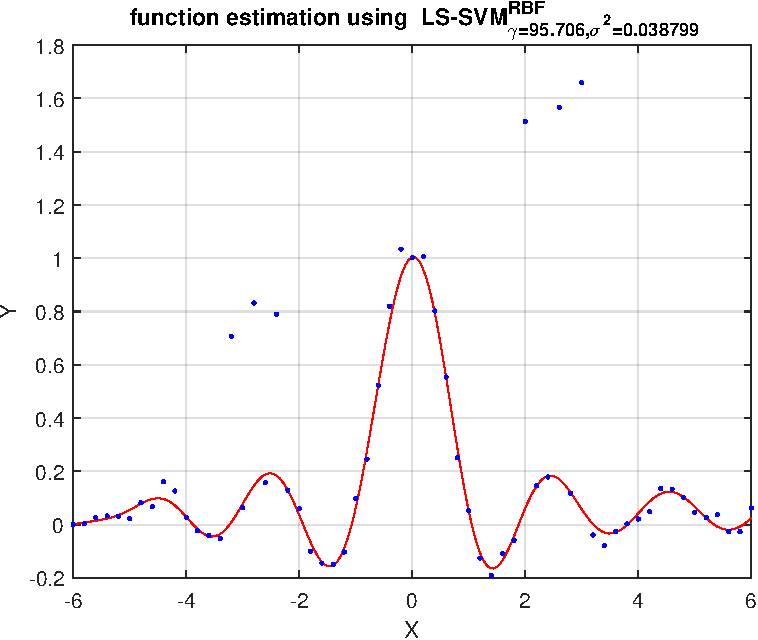
\includegraphics[width=\textwidth]{Assignment 2/figures/1_4/robust_mae_whuber.pdf}
                 \caption{MAE-Huber}
                 \label{fig:robust_regression_huber}
             \end{subfigure}
             \hfill
             %hampel
            \begin{subfigure}[b]{0.22\textwidth}
                 \centering
                 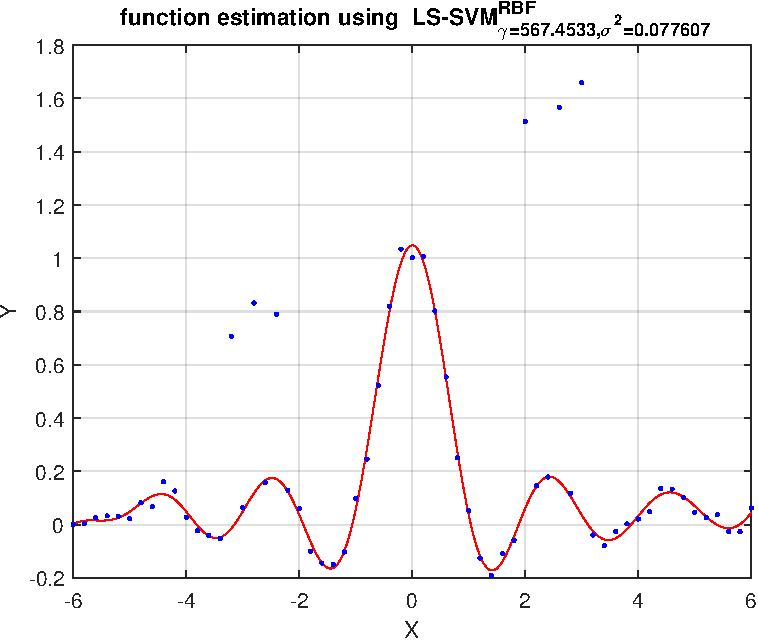
\includegraphics[width=\textwidth]{Assignment 2/figures/1_4/robust_mae_whampel.pdf}
                 \caption{MAE-Hampel}
                 \label{fig:robust_regression_hampel}
             \end{subfigure}
             \hfill
             %myriad
             \begin{subfigure}[b]{0.22\textwidth}
                 \centering
                 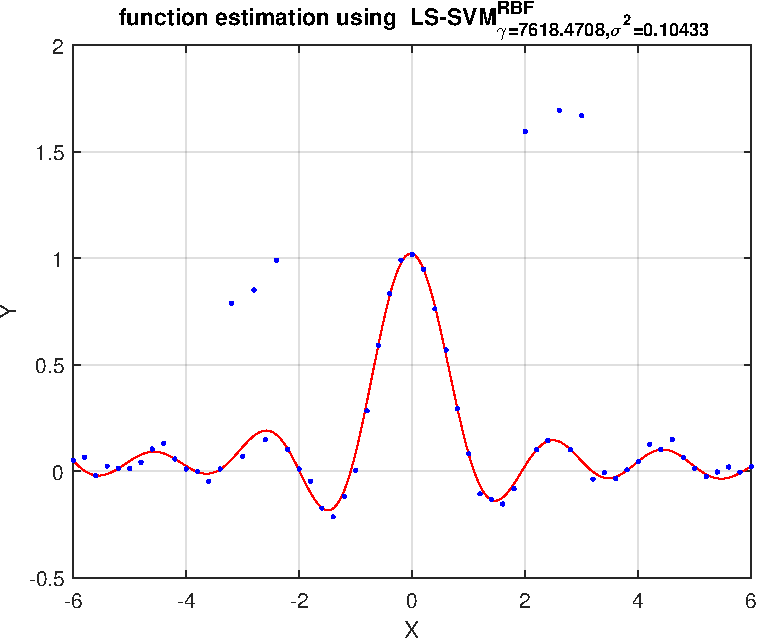
\includegraphics[width=\textwidth]{Assignment 2/figures/1_4/robust_mae_wmyriad.pdf}
                 \caption{MAE-Myriad}
                 \label{fig:robust_regression_myriad}
             \end{subfigure}
             \hfill
             %logistic
             \begin{subfigure}[b]{0.22\textwidth}
                 \centering
                 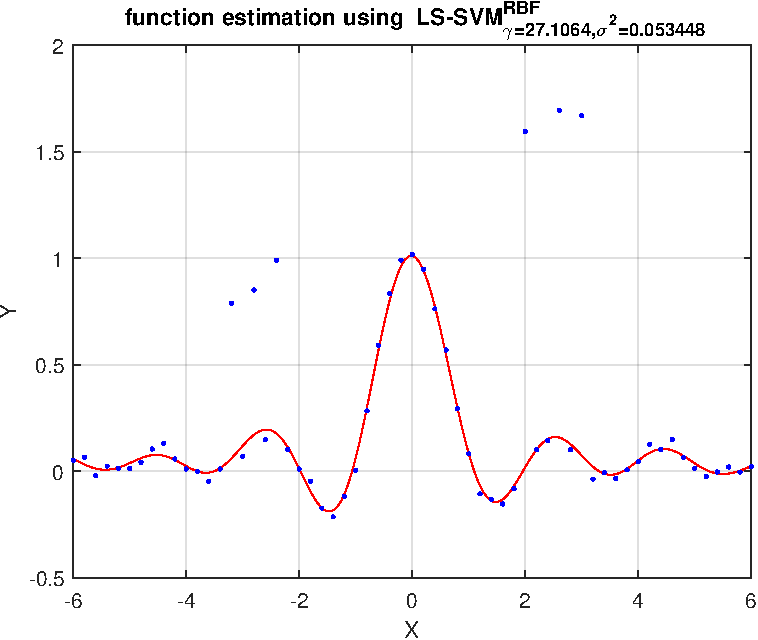
\includegraphics[width=\textwidth]{Assignment 2/figures/1_4/robust_mae_wlogistic.pdf}
                 \caption{MAE-Logistic}
                 \label{fig:robust_regression_logistic}
             \end{subfigure}
            \caption{Robust regression results for different weighting functions.}
        \end{figure}
    
\section{Homework problems}
    \subsection{Introduction: time series prediction}
        
        
        
    \subsection{Logmap dataset}
        % Time series prediction logmap
        \begin{figure}[h]
             \centering
             \hspace{0.05\textwidth}
             % Order tuning
             \begin{subfigure}[b]{0.4\textwidth}
                 \centering
                 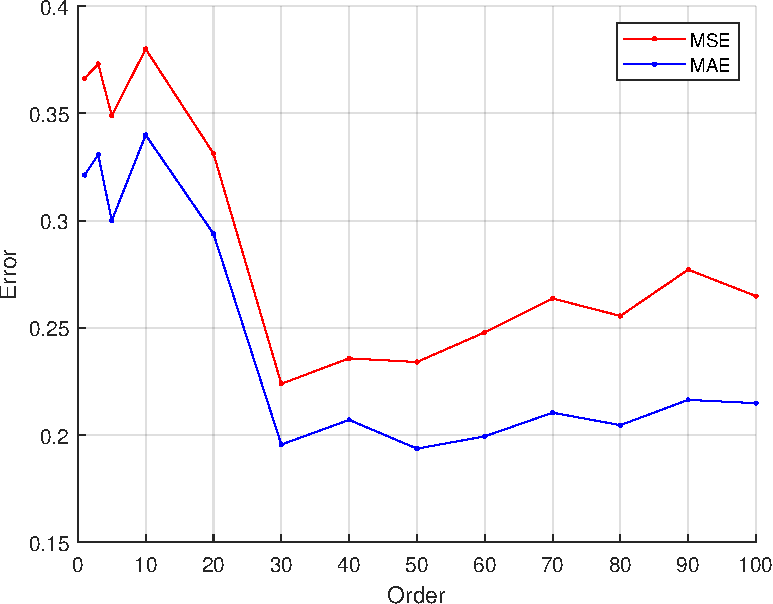
\includegraphics[width=\textwidth]{Assignment 2/figures/2_2/MSEvsMAE_ordersweep.pdf}
                 \caption{Errors for different orders.}
                 \label{fig:order_sweep}
             \end{subfigure}
             \hfill
            % Non robust
             \begin{subfigure}[b]{0.4\textwidth}
                 \centering
                 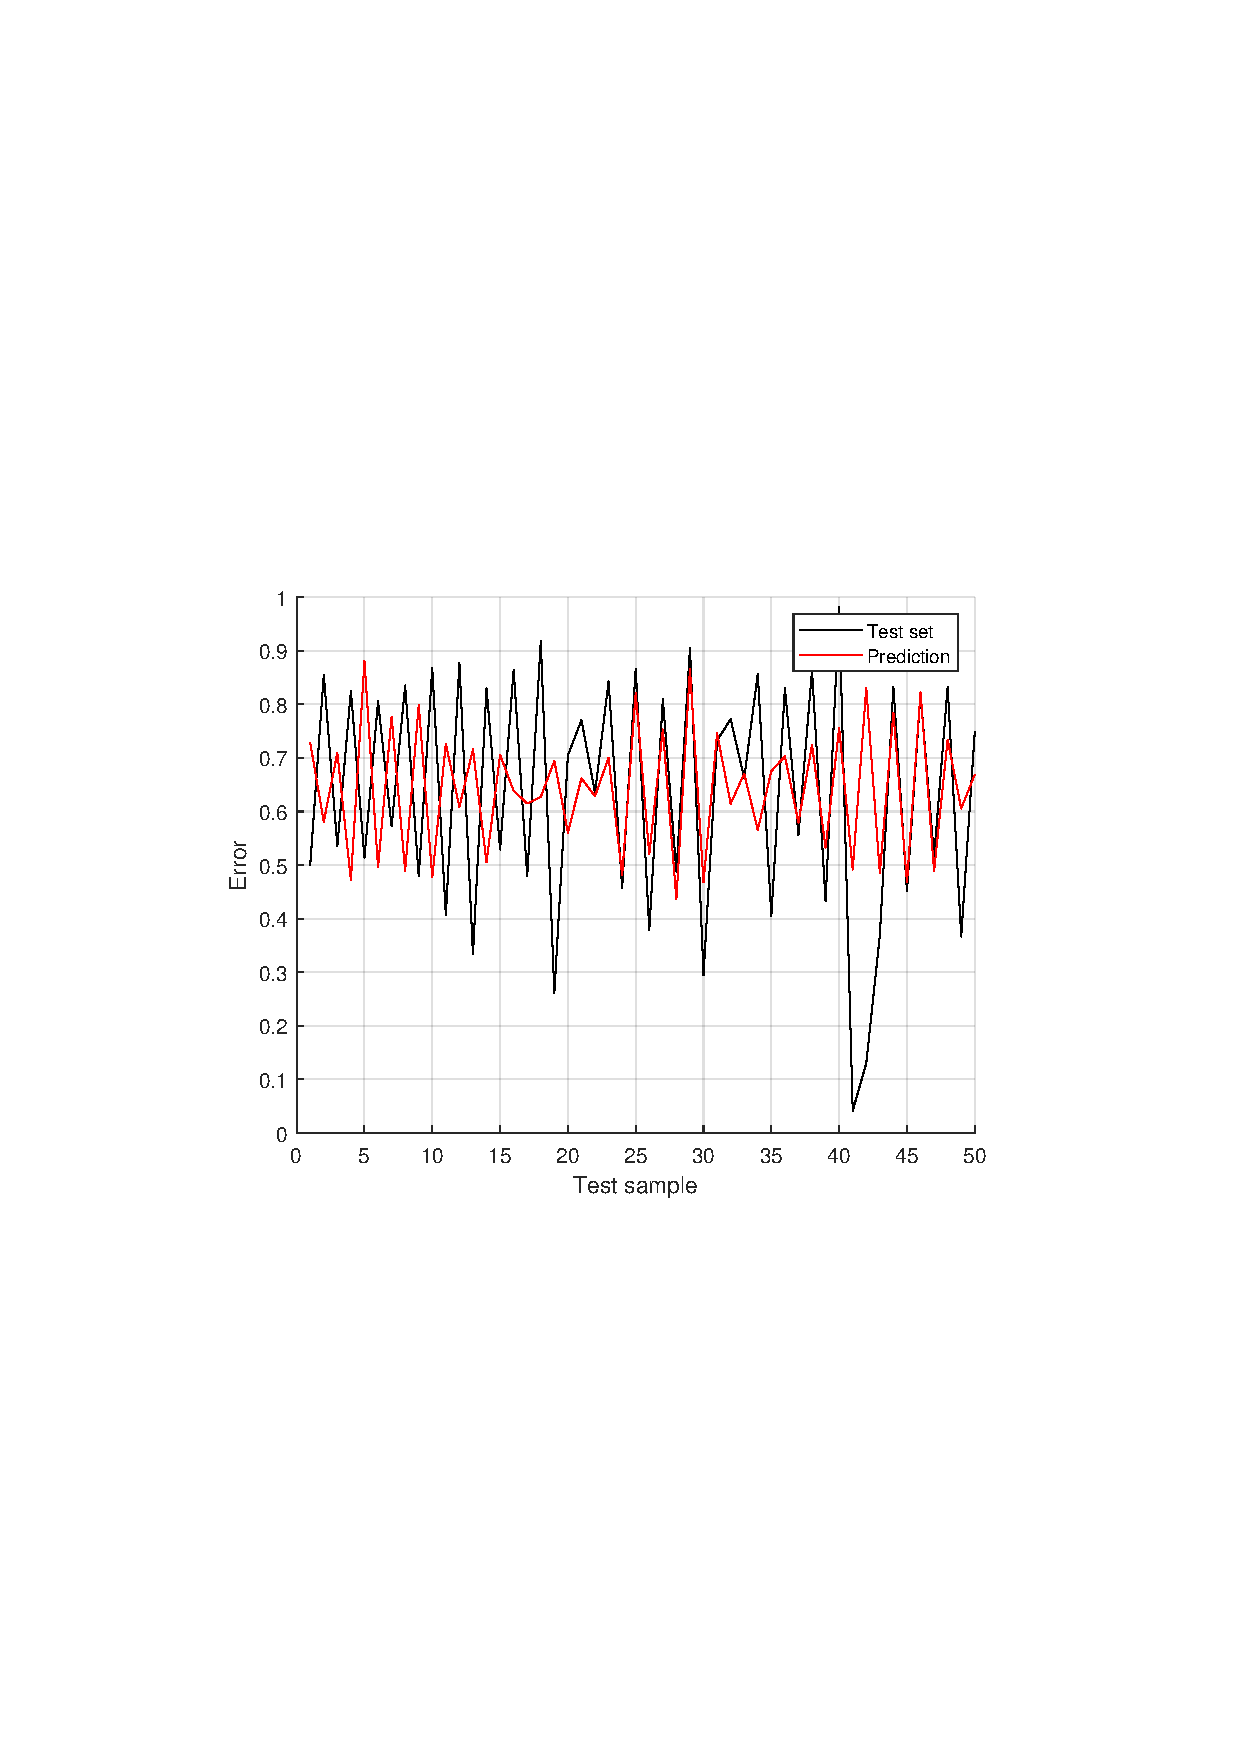
\includegraphics[width=\textwidth]{Assignment 2/figures/2_2/prediction.pdf}
                 \caption{Time series prediction result.}
                 \label{fig:logmap_prediction}
             \end{subfigure}
             \hspace{0.05\textwidth}
            \caption{Tuning (a) and prediction (b) results for time series regression on the Logmap dataset.}
        \end{figure}
    
        
        RMSE min =  0.2244
        min order = 30 
        
    \subsection{Santa Fe dataset}
        
        RMSE min =  19.22
        min order = 20
        
        % Time series prediction Santa Fe
        \begin{figure}[h]
             \centering
             \hspace{0.05\textwidth}
             % Order tuning
             \begin{subfigure}[b]{0.4\textwidth}
                 \centering
                 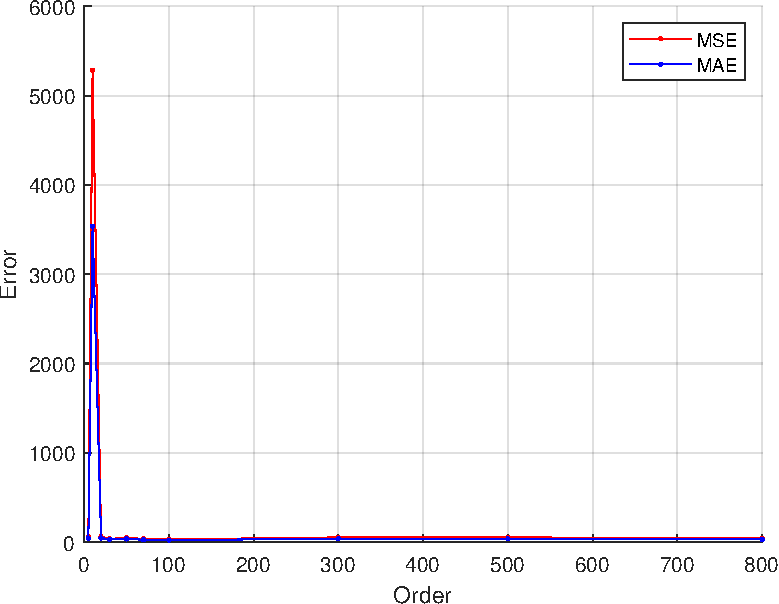
\includegraphics[width=\textwidth]{Assignment 2/figures/2_3/MSEvsMAE_ordersweep.pdf}
                 \caption{Errors for different orders.}
                 \label{fig:order_sweep_santa_fe}
             \end{subfigure}
             \hfill
            % Non robust
             \begin{subfigure}[b]{0.4\textwidth}
                 \centering
                 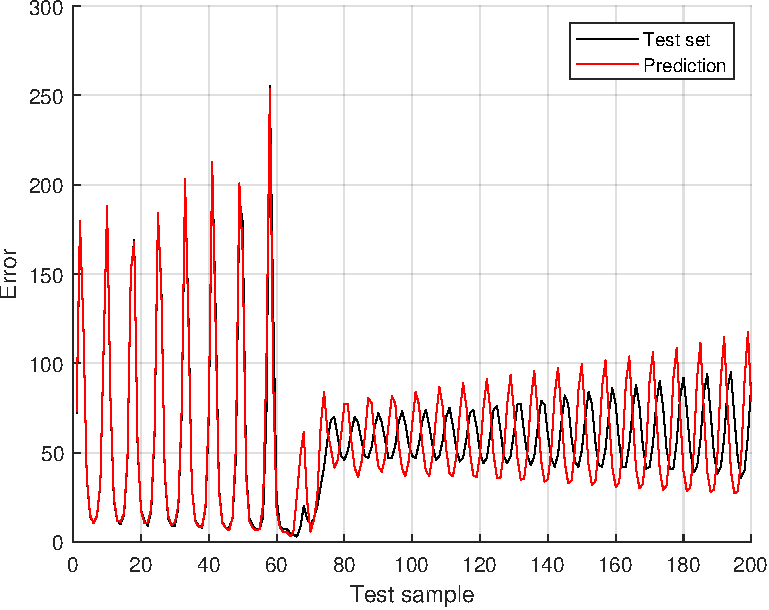
\includegraphics[width=\textwidth]{Assignment 2/figures/2_3/prediction_order_20.pdf}
                 \caption{Time series prediction result.}
                 \label{fig:santafe_prediction}
             \end{subfigure}
             \hspace{0.05\textwidth}
            \caption{Tuning (a) and prediction (b) results for time series regression on the Santa Fe dataset.}
        \end{figure}
        
    


\end{document}